\item \points{2e}
\textbf{Semi-supervised EM Implementation.}
Now we will consider both the labeled and unlabeled examples (a total of $\nexp + \tilde{\nexp}$), with 5 labeled examples per cluster. We have provided starter code for splitting the dataset into matrices \texttt{x} and \texttt{x\_tilde} of unlabeled and labeled examples respectively. Add to your code in |src-semi_supervised_em/submission.py| to implement the modified EM algorithm, and run it on the dataset until convergence.
More specifically, you will complete the |main| and |run_semi_supervised_em| functions. Note: feel free to create your own helper functions in the development of your solution.

Autograder test case |2e-1-basic| can be used to verify a correct implementation.  Before running the test case, change line 143 to |skip = False| (this test is skipped by default to make the autograder faster).  It will runcreate a plot for each trial, as done in the previous sub-question.

Your plots should look similar to the following (your plots are not graded):

  \begin{figure}[H]
    \centering
    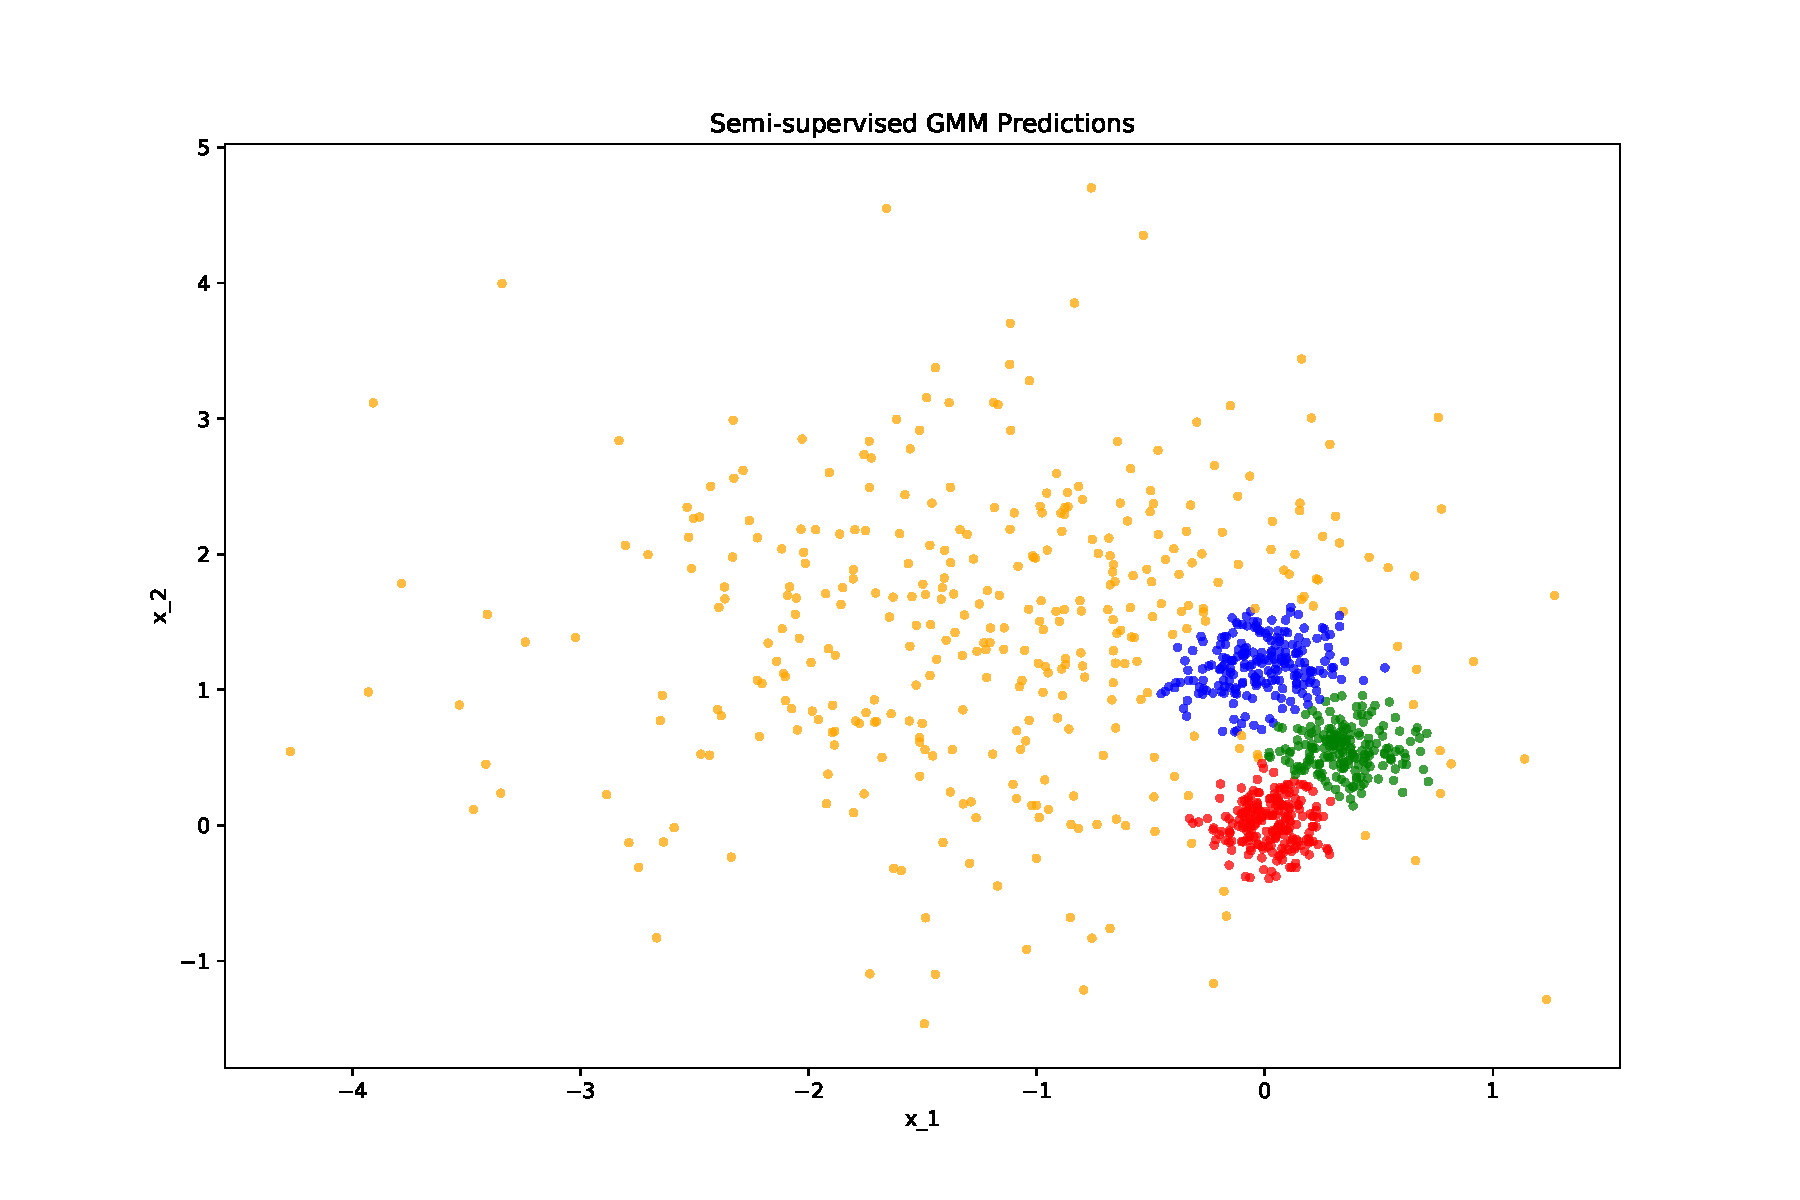
\includegraphics[width=0.3\textwidth]{02-semi_supervised_em/pred_ss_0.pdf}
    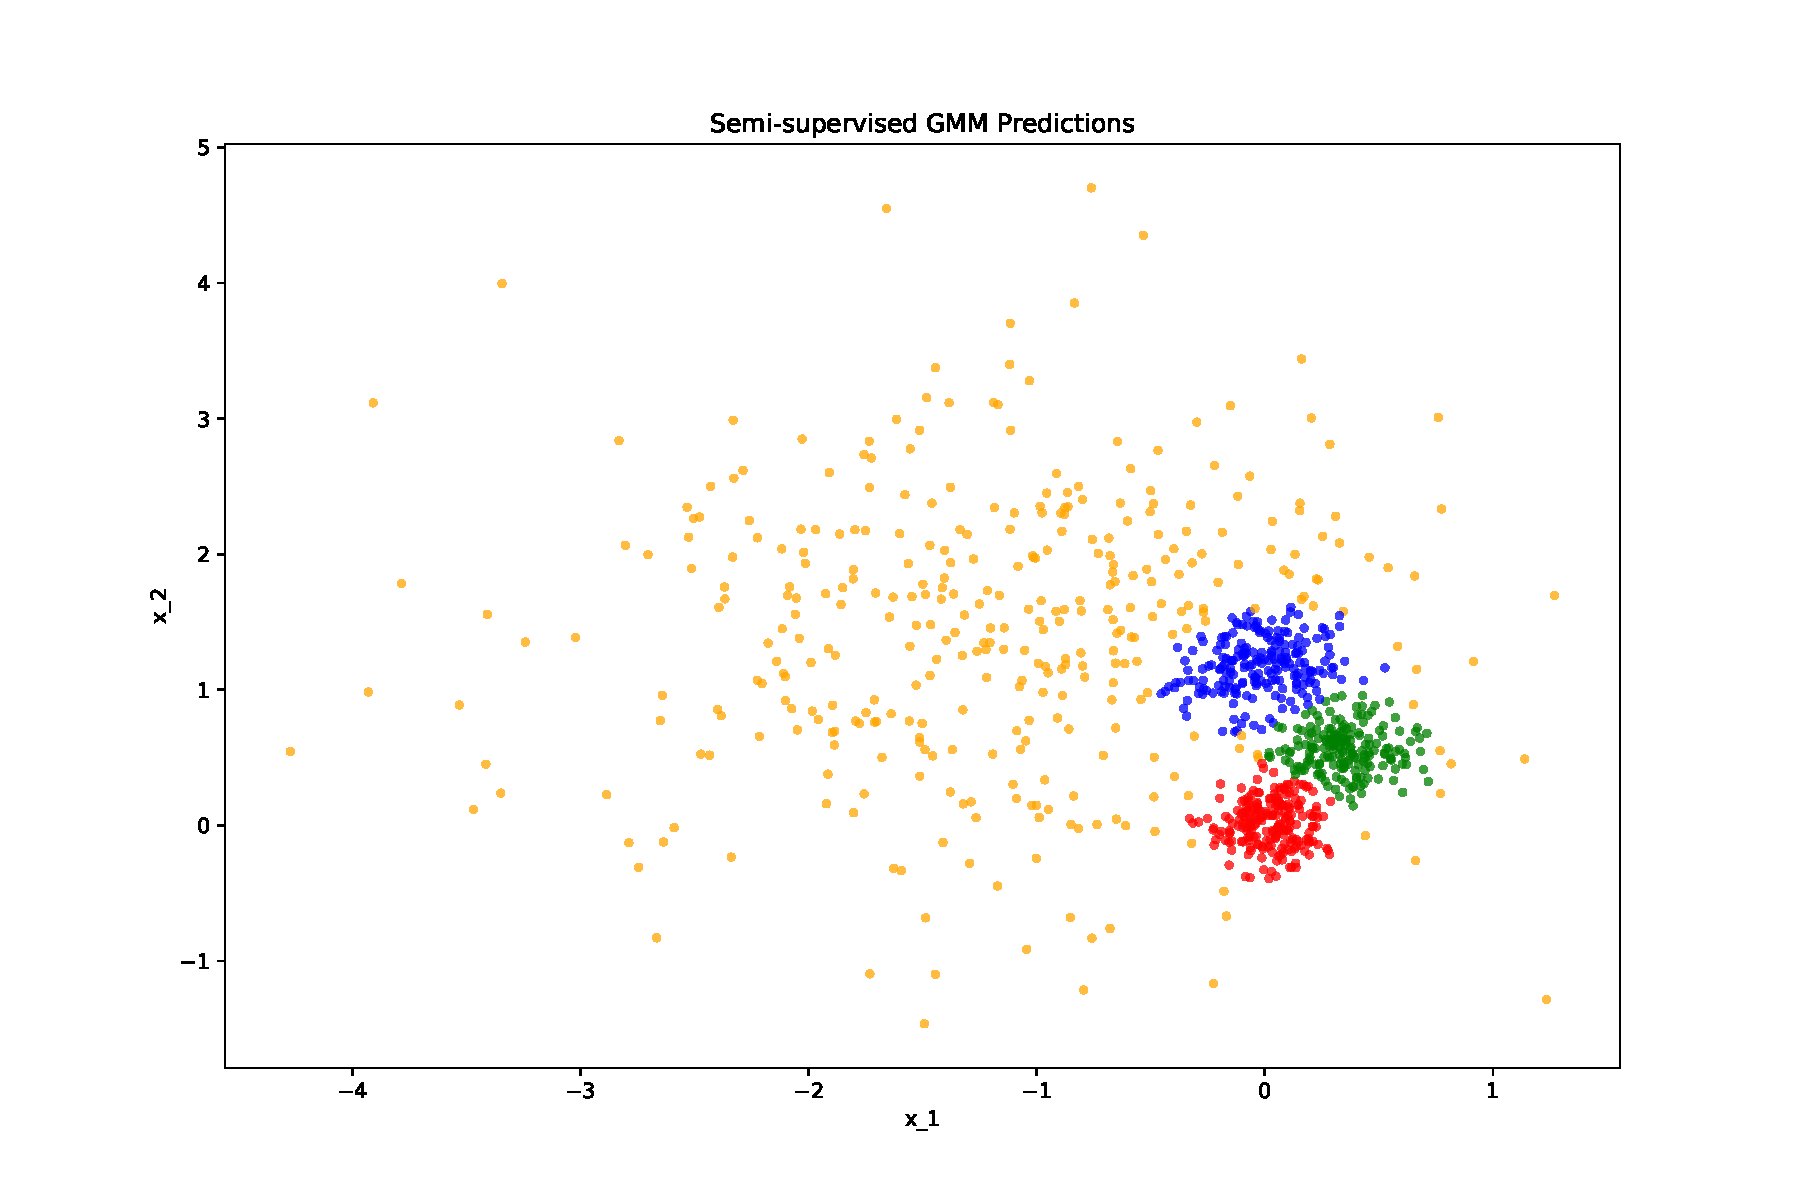
\includegraphics[width=0.3\textwidth]{02-semi_supervised_em/pred_ss_1.pdf}
    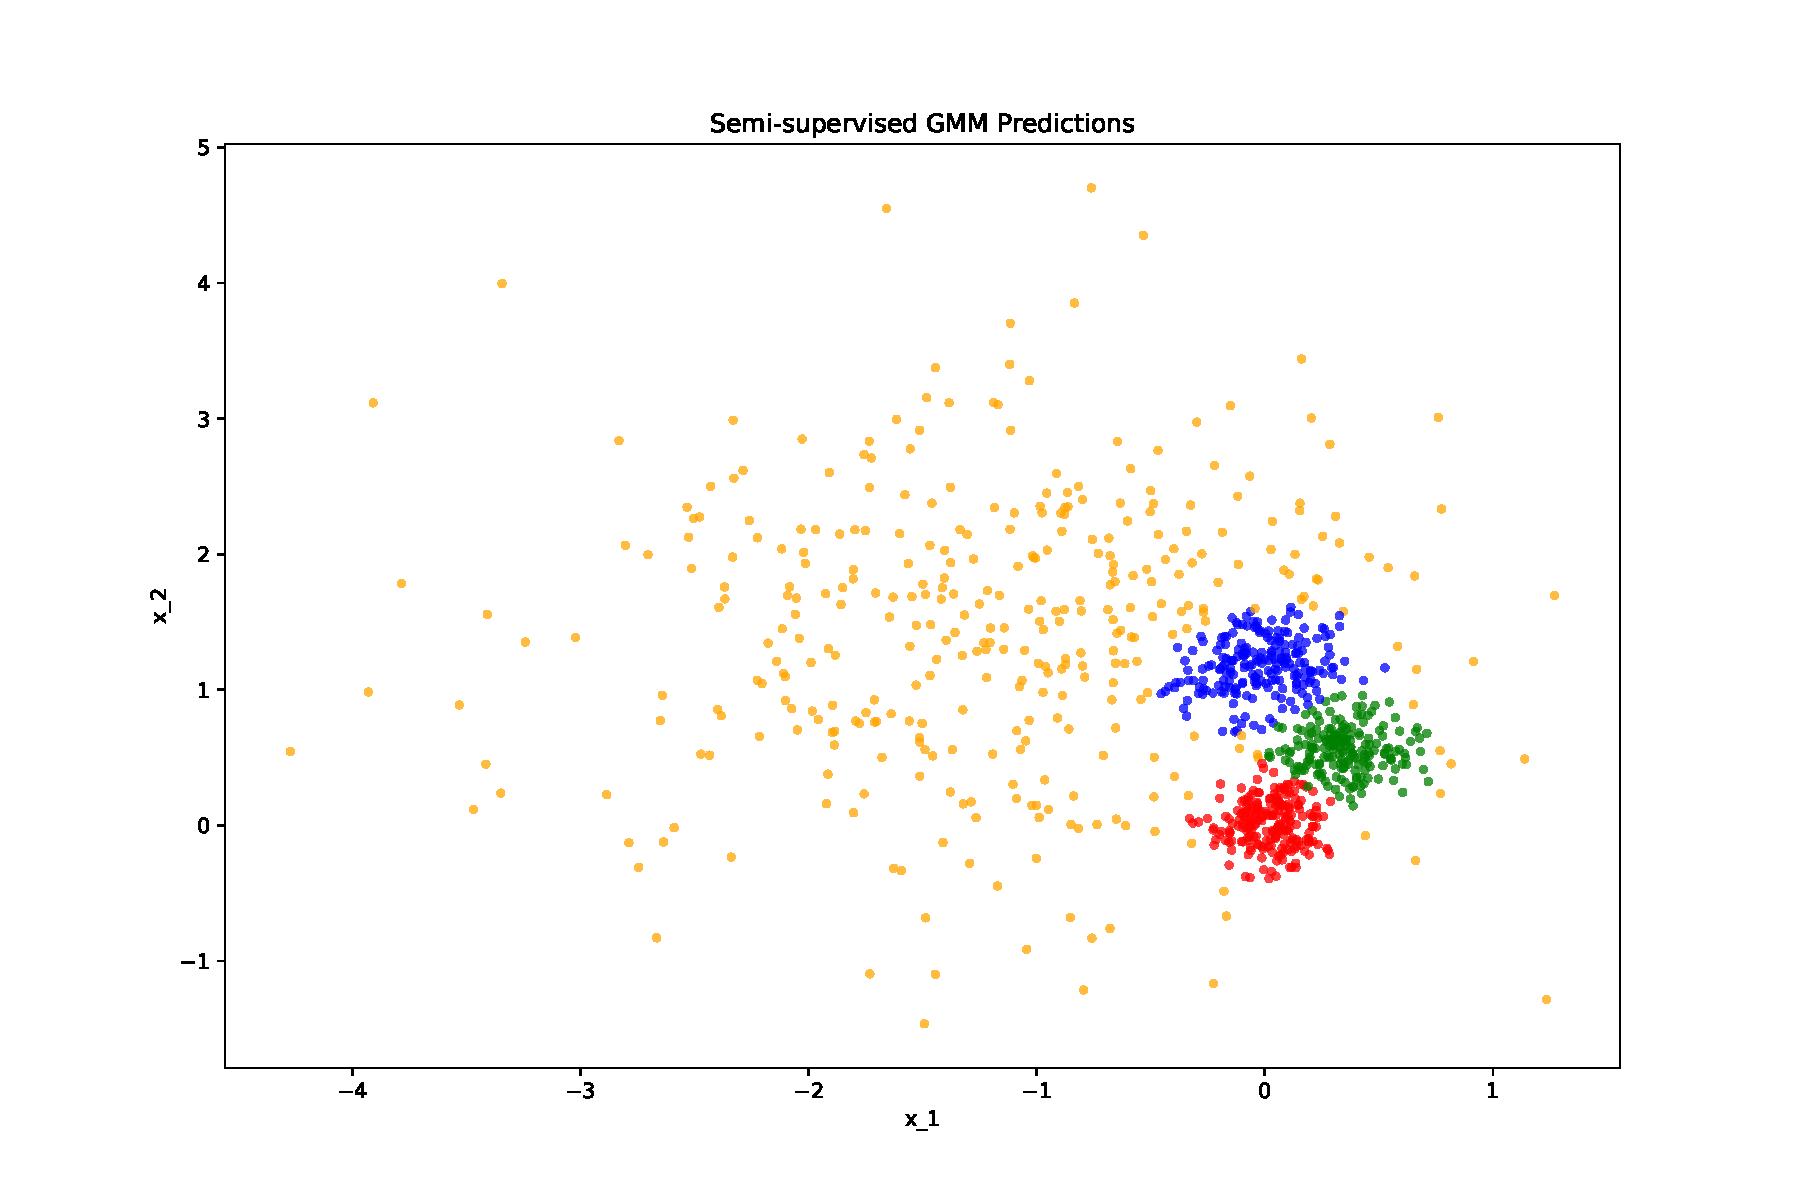
\includegraphics[width=0.3\textwidth]{02-semi_supervised_em/pred_ss_2.pdf}
    \caption{Predictions made by GMM model with semi-supervised EM.}
  \end{figure}
